%Start: 22/04/14
%Last edited on 02/05

%I sorted out the reference formatting by changing the encoding of my JabRef bibliography file
%Based on my outline for disparity paper_NC_April2014 notes

\documentclass[12pt,a4paper]{article}
\usepackage[round]{natbib} % author-year citations in round brackets


\raggedright %justify the text on the left only
\usepackage{enumerate} %put in numbers or bullet points

\usepackage{setspace}
\onehalfspacing %1.5 line spacing

\usepackage{authblk}%For author affiliations

\usepackage{graphicx} % For adding pictures

\usepackage{float}
\floatstyle{plaintop} %Force table captions to go above the table
\restylefloat{table} %allows you to force tables into specific places

\begin{document}

\title{Cranial morphological disparity within the adaptive radiation of tenrecs (Afrosoricida, Tenrecidae) is no greater than expected by chance} 

%I want to come up with a better title

\author[1,2,*]{Sive Finlay}
\author[1,2]{Natalie Cooper}
%Most likely put Steve in here as well

\affil[1]{School of Natural Sciences, and}
\affil[2]{Trinity Centre for Biodiversity Research, Trinity College Dublin, Dublin 2, Republic of Ireland}
\affil[*]{Corresponding author, sfinlay@tcd.ie}
\maketitle


\begin{abstract}

%I'll do this section last

\end{abstract}

\section{Introduction}

Understanding patterns of biological diversity remains a central challenge in evolutionary biology. Investigations of why some groups are more diverse than others help us to elucidate the patterns and underlying mechanisms governing the evolutionary success of a clade (REF). 

Many diverse groups such as Darwin's finches (REF), cichlid fish (REF), Caribbean \textit{Anolis} lizards (REF) and Hawaiian spiders (REF) are the products of adaptive radiations \citep{Losos2010}. Each of these groups are considered to be examples of exceptional diversity due to the variety of ecological niches which they occupy. 

The biological diversity of adaptively radiated groups can be characterised in two ways; species richness and phenotypic diversity. These metrics are generally decoupled during adaptive radiations; taxonomic diversity does not necessariliy correlate with phenotypic variety \citep{Ruta2013, Hopkins2013}. 
However, taxonomic diversity is not a pre-requisite for characterising a group as being the product of an adaptive radiation \citep{Losos2010}. In contrast, adaptive radiation refers to the diversification of an ancestral species into descendants which are adapted to a variety of ecological niches \citep{Losos2010a}. Clades that have exceptional phenotypic diversity can still be considered adaptive radiations even if they are not taxonomically diverse. Therefore it is important to quantify phenotypic diversity explicitly to determine whether there is evidence for adaptive radiation in a clade.

Phenotypic diversity is commonly measured as morphological disparity; the diversity of organic form \citep{Foote1997,Erwin2007}). Palaeontological studies often use disparity as an index of evolutionary patterns over time \citep[e.g.][]{Brusatte2008, Ciampaglio2001, Wills1994} but studies of disparity in extant taxa are also becoming increasingly common \citep[e.g.][]{Harmon2003, Collar2011}. 

There is no single definition of disparity and it is calculated using multiple metrics, each of which describe different aspects of morphological variation \citep{Ciampaglio2001}. Many metrics measure disparity as the area of morphospace occupied by a particular group; clades with higher disparity will occupy greater areas of morphospace \citep[e.g.][]{Goswami2011, Brusatte2008}. Alternative approaches identify disparity as a function of both the rate of evolution and phylogenetic topology of a clade \citep{OMeara2006}. This view focuses on morphological change over time where faster rates correspond to greater morphological evolution over a given time and therefore higher disparity \citep{Price2013}. 
These two approaches characterise different views of disparity. Metrics based on morphospace variation measure disparity as the amount of variation in morphological form while rate-based approaches quantify disparity as the amount of directed change away from an ancestor \citep{Zelditch2012}.

\textit{I need to finish off the paragraph here depending on whether I end up using one or both approaches} 


%Remember that I need to put in something about extinction too - either here or in the discussion

Here we test whether there is evidence for significant morphological disparity in an adaptive radiation of small insectivore mammals.

Tenrecs (Afrosoricida, Tenrecidae) are comprised of 34 species, 31 of which are endemic to Madagascar \citep{Olson2013}. The extant Malagasy tenrecs evolved from a single common ancestor \citep{Asher2006} which is thought to have colonised the island between 25 and 42 million years ago \citep{Samonds2013}. This ancestor diversified into a wide variety of descendant species which convergently resemble distantly related insectivore mammals such as shrews (the \textit{Microgale} tenrecs), moles (\textit{Oryzorictes} tenrecs) and hedgehogs (\textit{Echinops,Setifer} tenrecs) \citep{Eisenberg1969}.

Tenrecs are often cited as an example of an adaptively radiated family which exhibits exceptional morphological diversity \citep{Soarimalala2011, Olson2003, Eisenberg1969}
%Losos2010a; adaptive radiation should be reserved for those clades exhibiting exceptional ecological and phenotypic disparity


However, this apparent exceptional diversity is based on subjective comparisons to other groups and it has not been tested quantitatively. Losos and Mahler \citeyearpar{Losos2010a} argue that the term adaptive radiation should only be applied to clades exhibiting exceptional (i.e. greater than expected by chance) ecological and phenotypic diversity.
Here we address one of these two criteria and test whether the apparent phenotypic diversity exhibited by tenrecs represents an exceptional example of morphological disparity. 

If tenrecs are exceptionally morphologically diverse there are two predictions \citep{Losos2010a}:   
\begin{enumerate}
\item Tenrecs are more morphologically disparate than expected by chance
\item Tenrecs show a significantly higher level of disparity than their closest relatives, the golden moles (Afrosoricida, Chrysochloridae)
\end{enumerate}

Using the most complete morphological data set of tenrecs and golden moles to date (n=43 species, 31 tenrecs and 12 golden moles) we apply geometric morphometric analyses \citep{Rohlf1993, Zelditch2012} to quantify morphological disparity among our species. Given that there is no single best method to quantify disparity \citep{Ciampaglio2001} we calculate and compare multiple disparity metrics (REFS) for our data. We compare morphological disparity of tenrecs to both simulated data (prediction 1) and the disparity of their nearest relatives (prediction 2).

Surprisingly we find that, despite initial appearances, tenrecs are not more morphologically diverse than expected by chance. This result still holds when disparity is calculated without the highly phenotypically similar and speciose (19 of the total 31 tenrec species) genera of \textit{Microgale} (shrew-type) tenrecs.

Furthermore, when compared to golden moles, tenrecs have a higher level of disparity in the shape of their skulls but not in their mandibles, indicating that tenrecs are more phenotypically diverse in some but not all aspects of their morphologies.

Our results indicate that, on average, tenrecs are more phenotypically diverse than their closest relatives but their morphological diversity is no greater than that which is expected to evolve by chance. Therefore, under strict definitions, their designation as an exceptional adaptive radiation may need to be reconsidered. 

These findings highlight the vital importance of testing our common but often eroneous expectations about patterns of morphological diversity in adaptively radiated groups. 

%I need a better final sentence here

\section{Methods}
To quantify morphological disparity in tenrecs and their closest relatives, the golden moles (Chrysochloridae), we used a combination of geometric morphometric techniques and phylogenetic comparative methods. 

\subsection{Taxonomy and Phylogeny}
We used the most up to date mammalian taxonomy \citep{Wilson2005} as a guide for identifying our specimens. However it was also necessary to supplement this information with more recent sources \citep{IUCN2012, Olson2013} to account for the additional species of \textit{Microgale} tenrec \citep{Olson2004, Goodman2006, Olson2009} which are now recognised. 

%maybe take out this last bit since I only have one of the 4 new Microgale species (M.jobihely) in my dataset?

Instead of basing our analyses on individual trees and assuming that their topology were known without error 
%I got this line from the longevity paper!
\citep[e.g.][]{Ruta2013, Foth2012, Brusatte2008, Harmon2003} we used a distribution of 101 pruned phylogenies derived from the randomly resolved mammalian supertrees in \citep{Kuhn2011}. 
There were 8 species (6 \textit{Microgale} tenrecs and 2 golden moles) in our morphological data which were not in the phylogenies. Phylogenetic relationships among the \textit{Microgale} have not been resolved more recently than the \citep{Kuhn2011} analysis, therefore we added the additional \textit{Microgale} species at random to the \textit{Microgale} genus within each phylogeny \citep{Revell2012}. We could not use the same approach to add the two missing golden mole species because they were the only representatives of their respective genera within our data. Therefore we added these species at random to the common ancestral node (findMRCA function in phytools \citep{Revell2012}) of all golden moles within each phylogeny. Adding these extra species to the phylogenies created polytomies which we resolved at random \citep{Paradis2004}. We calculated pairwise phylogenetic distances among species using the cophenetic function \citep[R Development Core][]{Team2013}. 


\subsection{Geometric Morphometrics}

Due to the high number and relatively small sizes of our specimens we chose to use two dimensional morphometrics rather than 3D techniques. We photographed cranial specimens of tenrecs and golden moles at five different institutions; the Natural History Museum London (NHML), the Smithsonian Institute Natural History Museum (SI), the American Museum of Natural History (AMNH), Harvard's Museum of Comparative Zoology (MCZ) and the Field Museum of Natural History, Chicago. We photographed the specimens with a Canon EOS 650D camera fitted with an EF 100mm f/2.8 Macro USM lens. We used a standardised procedure to minimise potential variability or error that could be associated with obtaining the pictures (see the supplementary material for details).
%I haven't written the supplementary material yet
We collected pictures of the skulls in dorsal, ventral and lateral views (right side of the skull) and of the outer (buccal) side of the right mandibles. A full list of museum accession numbers and corrected taxonomy can be found in the supplementary material and photographs of the specimens are on figshare (http://dx.doi.org/10.6084/m9.figshare.705863).\\
%I only have the AMNH and SI pictures on figshare because the other insitutions were more touchy about copyright

We collected data from 31 species of tenrec (out of the total 34 in the family) and 12 species of golden moles (out of a total of 21 in the family \citep{Asher2010}). Our sample sizes were pictures of 182 skulls in dorsal view (148 specimens of tenrecs and 34 specimens of golden moles) and 181 mandibles in lateral view (147 specimens of tenrecs and 34 specimens of golden moles).
	
Although morphometric studies are well suited to extremely detailed investigations of shape variation in closely related taxa \citep[e.g.][]{Cardini2003, Panchetti2008, Blagojevic2011}, there is increasing interest in using morphometrics for more broad scale, cross-taxonomic analyses \citep{Wroe2007, Klingenberg2013}. Our study falls into the later of these two groups. We were interested in changes in overall cranial shape among the 43 species of tenrecs and golden moles rather than specific differences between corresponding homologous anatomical features. Therefore we used a combination of both landmarks (type 2 and type 3, \citep{Zelditch2012}) and semilandmarks to characterise the shapes of our specimens.

To guide our landmark selection for each of the data sets we used existing studies of both morphological (not morphometric) variation in our study species \citep{Asher1999, Asher2008, Asher2010} and unrelated taxa \citep[e.g.][]{Barrow2008, Panchetti2008, Macholan2008, Klenovsek2013}. 
Here we present our landmarks (points) and semilandmarks (outline curves) used to represent shape variation in the dorsal skulls and mandibles (Figures \ref{dorslandmarks} and \ref{mandslandmarks}).

Corresponding landmark definitions for each view are in tables \ref{dorslanddesc} and \ref{mandslanddesc}.

%These figures still look rough
	%Most papers have pictures which look like diagrams - drawings rather than photos - but I need to work out how to do that. Thomas might have a few ideas?

\begin{figure}[H]
\centering
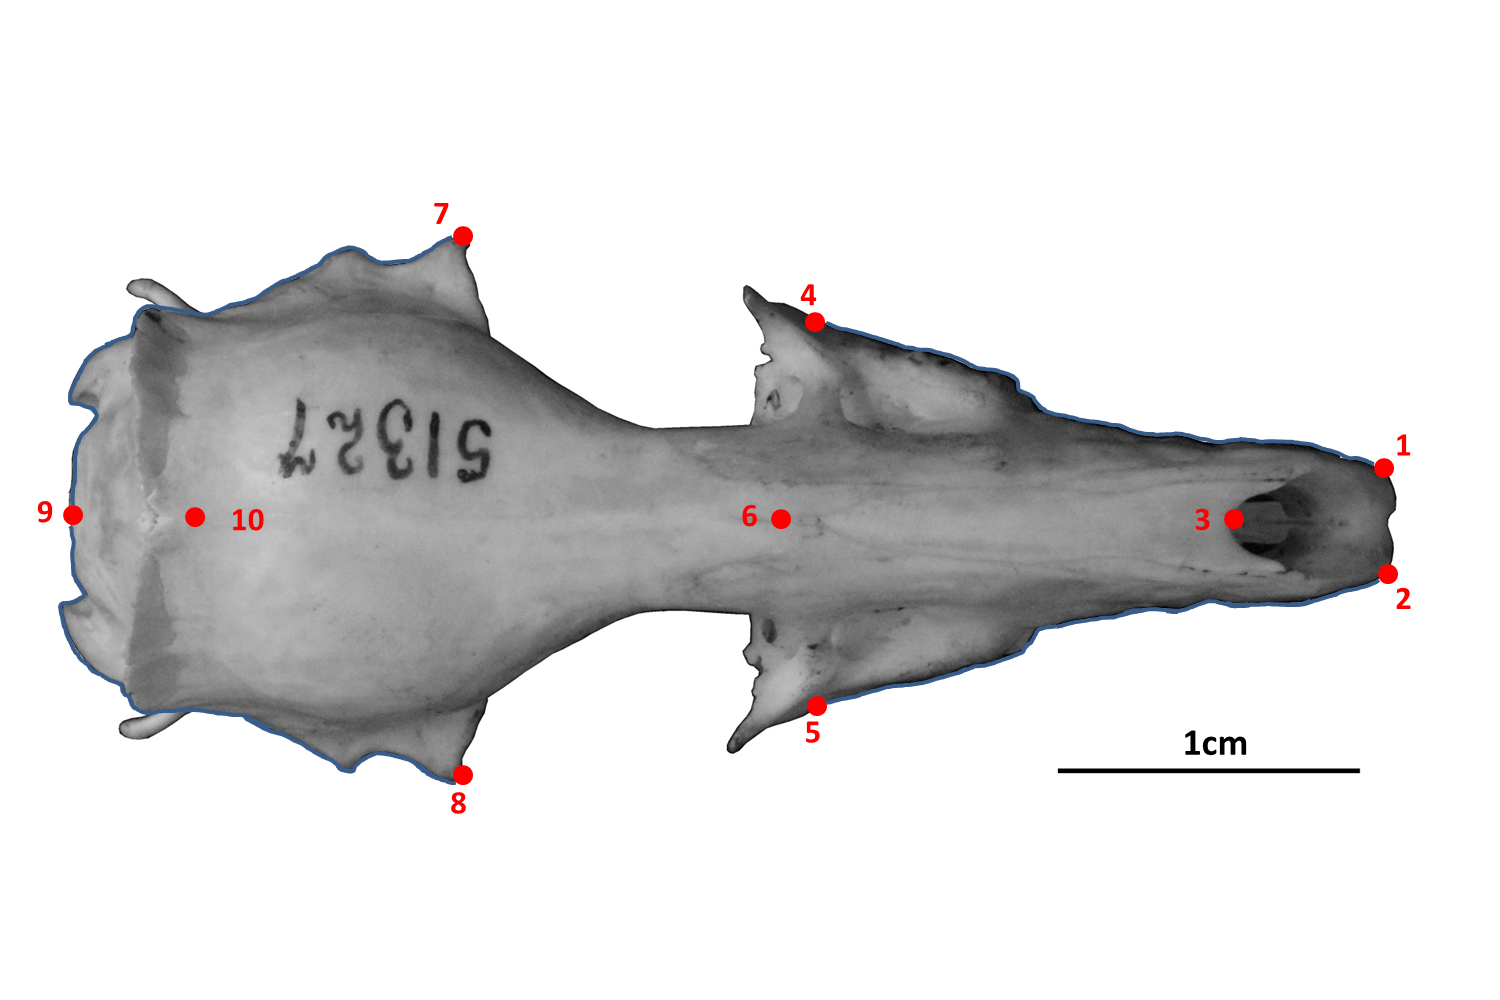
\includegraphics[width=1\linewidth]{AMNH_51327_dorsallandmarksdiagram.png}
\caption{Landmarks (red points) and curves (blue lines) used to capture the morphological shape of skulls in dorsal view. Curves were re-sampled to the same number of evenly-spaced points. See table X for description of curves and landmarks.\textit{Potamogale velox} (Tenrecidae) skull, museum reference number AMNH\_51327}
\label{dorslandmarks}
\end{figure}


%Table for the dorsal skulls landmark descriptions

\begin{table}[H]			
\centering
\caption{Descriptions of the landmarks (points) and curves (semilandmarks) for the skulls in dorsal view (see Figure \ref{dorslandmarks}).}
\begin{tabular}[t]{l l}		
\hline
\textbf{Landmark} & \textbf{Description} \\
\hline
1 + 2 & Left (1) and right (2) anterior points of the premaxilla \\
3 & Anterior of the nasal bones in the midline \\
4 + 5 &	Maximum width of the palate (maxillary) on the left (4) and right (5)\\
6 & Midline intersection between nasal and frontal bones \\
7 + 8 & Widest point of the skull on the left (7) and right (8) \\
9 &	Posterior of the skull in the midline \\
	%Panchetti 2008 and Macholan2008 have different definitions for this one so I need to choose one
10 & Posterior intersection between saggital and parietal sutures \\

\hline
\textbf{Curves} & \textbf{Description}\\
\hline

\textbf{Curve A} & Outline of the braincase on the left side, between landmarks 9 and 7\\ 
(12 points) & (does not include visible features from the lower (ventral) side of the skull) \\

\textbf{Curve B} & Outline of the palate on the left side, between landamarks 4 and 1 \\
(10 points) & (outline of the rostrum only, not the shape of the teeth)\\

\textbf{Curve C} &	Outline of the braincase on the right side, between landmarks 9 and 8 \\
(12 points) & (does not include visible features from the lower (ventral) side of the skull) \\

\textbf{Curve D} & Outline of the palate on the right side, between landamarks 5 and 2 \\
(10 points) & (outline of the rostrum only, not the shape of the teeth)\\

\hline
\end{tabular}
\label{dorslanddesc} %give it a label so I can refer to it in the text
\end{table}

\begin{figure}[H]
\centering
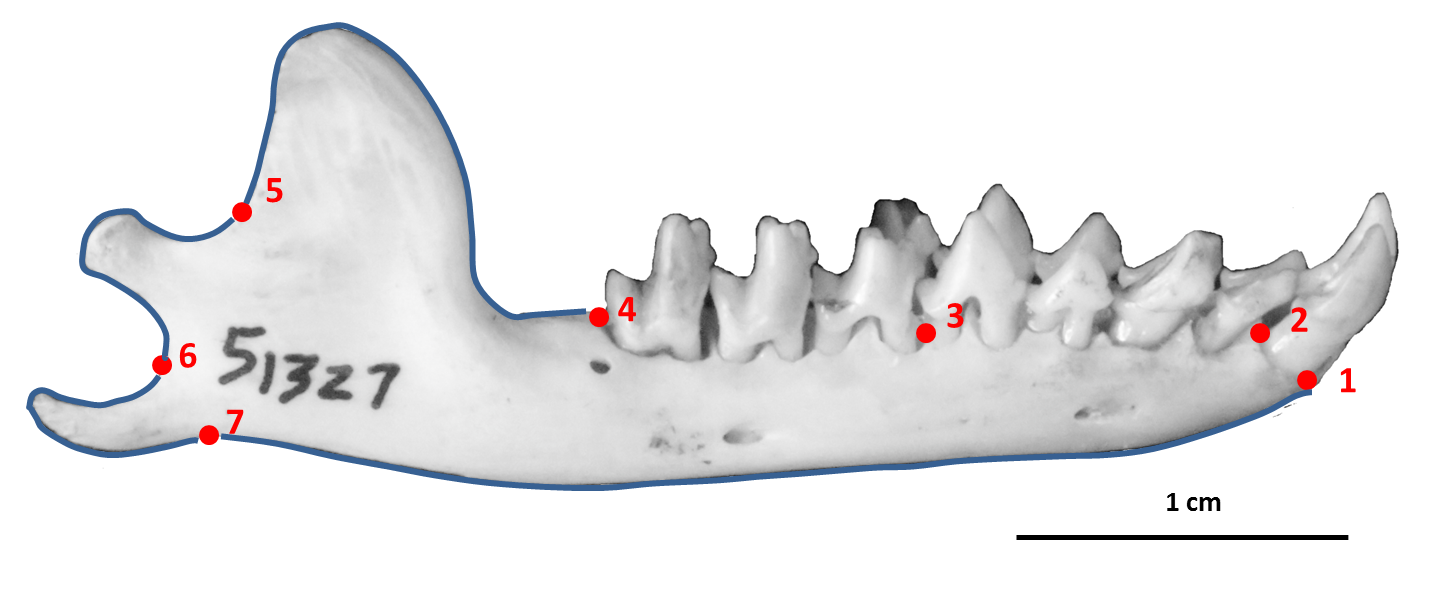
\includegraphics[width=1\linewidth]{AMNH_51327_landmarksdiagram.png}

\caption{Landmarks (red points) and curves (blue lines) used to capture the morphological shape of mandibles. Curves were re-sampled to the same number of evenly-spaced points. See table X for description of curves and landmarks.\textit{Potamogale velox} (Tenrecidae) mandible, museum reference number AMNH\_51327}
\label{mandslandmarks}
\end{figure}

%Table for the mandibles' landmark descriptions

\begin{table}[H]			
\centering
\caption{Descriptions of the landmarks (points) and curves (semilandmarks) for the mandibles in lateral (buccal) view (see figure \ref{mandslandmarks})}
\begin{tabular}[t]{l l}		
\hline
\textbf{Landmark} & \textbf{Description} \\
\hline
1 & Anterior of the alveolus of the first incisor \\
2 & Posterior of the alveolus of the first incisor \\
3 &	Anterior of the alveolus of the first molar \\
4 & Posterior of the alveolus of the last molar \\
5 & Point of maximum curvature between the coronoid and condylar processes \\
6 & Point of maximum curvature between the condylar and angular processes  \\
7 &	Point of maximum curvature between teh angular process and the horizontal ramus \\

\hline
\textbf{Curves} & \textbf{Description}\\
\hline

Curve A & Shape of the condyloid process (between landmarks 4 and 5, 15 semilandmarks) \\
Curve B & Shape of the condylar process (between landmarks 5 and 6, 15 semilandmarks) \\
Curve C & Shape of the angular process (between landmarks 6 and 7, 15 semilandmarks) \\
Curve D & Shape of the base of the jaw (between landmarks 7 and 1, 12 semilandmarks \\
\hline
\end{tabular}
\label{mandslanddesc} %give it a label so I can refer to it in the text
\end{table}
 
Our analyses of ventral and lateral skull views yielded similar patterns in our disparity analyses (see results), details can be found in the supplementary material. We digitised all landmarks and semilandmarks in tpsDIG, version 2.17 \citep{Rohlf2013}.

%Diagram of the dorsal and mandible landmarks
%Table of the landmark definitions


We re-sampled the outlines to a standard number of evenly spaced points which were the minimum number required to represent each outline accurately \citep[][details in supplementary material]{MacLeod2013}. We used TPSUtil \citep{Rohlf2012} to create sliders files \citep{Zelditch2012} which defines which points are semilandmarks. We conducted all subsequent analyses in R version 3.0.2 \citep[R Development Core][]{Team2013} within the geomorph package \citep{Adams2013}. We used the gpagen function to run a general Procrustes alignment (REFS) of the landmark coordinates while sliding the semilandmarks by minimising procrustes distance rather than bending energy (REFS). We used these Procrustes-aligned coordinates of all species (n=43) to calculate average shape values for each species which we then used for a principal components analysis (REFS) with the plotTangentSpace function \citep{Adams2013}.  We used the principal component axes which cumulatively accounted for 95\% of the variation in each data set (REFS - maybe the Brusatte ones?)  to calculate morphological disparity.




\subsection{Disparity calculations} 


We calculated disparity separately for golden moles and tenrecs in each of the morphological datasets. We used the PC axes which accounted for 95\% of the cumulative variation to calculate four disparity metrics; the sum and product of the range and variance of morphospace occupied by each family \citep{Brusatte2008, Foth2012, Ruta2013}. We also calculated morphological disparity directly from the Procrustes-superimposed shape data \citep{Zelditch2012}. 

To test our first prediction; tenrecs are more morphologically disparate than expected by chance, we simulated shape evolution  \citep{Harmon2008} of the species-average, Procrustes-superimposed shape coordinates of each tenrec species across our distribution of phylogenies under a Brownian Motion (BM) model (1000 simulations on each of 101 phylogenies pruned to include tenrec species only). We ran a principal components analysis on each of the simulations and used the PC axes which accounted for 95\% of the cumulative variation to calculate disparity metrics.
 
%I still need to calculate the Zelditch metric for each of the simulations

We compared the observed disparity measure to the corresponding distribution of values and used a two tailed test to determine whether the observed (true) disparity measures were more or less than expected by chance.

The majority of tenrecs (19 out of 31 in our data) are members of the \textit{Microgale} (shrew-like) genus which is notable for its relatively low phenotypic variety \citep{ Soarimalala2011, Jenkins2003}. Therefore we hypothesised that phenotypic similarity among these species may mask signals of high disparity among other tenrecs. To test this idea, we repeated our simulations of shape evolution in non-\textit{Microgale} tenrec species only. This reduced our data from 31 to 12 species and the number of specimens from 148 (all tenrecs) to 53 (non-\textit{Microgale}) skulls and from 147 to 54 mandibles. We pruned the tenrec phylogenies to remove the \textit{Microgale} for these reduced simulations. We compared the observed disparity of non-\textit{Microgale} tenrecs to the distributions of the expected disparity from our simulations. 


To address our second prediction; tenrecs are more disparate than their nearest relatives, we used a non parametric MANOVA \citep{Anderson2001} to compare morphospace occupation between the two groups (REFS?). 

Our data includes more tenrec speices and specimens than golden moles and disparity is expected to be higher in larger groups (REFS). Therefore, we repeated our group comparisons of disparity within rarefaction analyses (see supplementary material) to confirm that observed differences in disparity between the two groups were not artefacts of differences in sample size.



\section{Results}

\subsection{Morphological disparity in tenrecs is not greater than expected by chance}

We compared observed disparity to calculations of disparity from BM simulations of shape data (101,000 simulations across 101 phylogenies). For each metric of disparity in both the dorsal skulls' (table \ref{skdorssims}) and mandibles' morphologies (table \ref{mandssims}), the true (observed) values were significantly lower than expected compared to the distribution of simulated values. We also found significantly lower disparity than expected by chance in both the ventral and lateral skull views (supplementary material).

Removing the phenotypically similar \textit{Microgale} tenrecs did not make a difference to our results; the non-\textit{Microgale} tenrecs still show significantly lower phenotypic disparity than expected by chance (simulation results in the supplementary material). 


%Table of the simulation results for SkDors tenrecs
	%comes from the SkDors_Trc+Gmole_TenrecDisparity_1000simsOutput file

\begin{table}[H]				%h places the table where it's neatest at that point in the code

\centering
\caption{Comparison of observed and simulated disparity measures for the dorsal skulls analysis; observed (true) disparity measures, minimum simulated value (sim.min), maximum simulated value (sim.max), standard deviation of the simulated values (sdev.sim) and p value comparing the observed disparity measures to the distribution of simulated values)}

\begin{tabular}[t]{l l l l l l }		%l left aligns p gives defined col width for long entries
\hline
%\
\textbf{Disparity metric} & \textbf{Observed} & \textbf{Sim.min} & \textbf{Sim.max} & \textbf{Sdev.sim} & \textbf{p value} \\
%\multicolumn{6}{c}{}\\	% empty line below the column headers
\hline
Sum of Variance & 0.0017 & 24742.44 & 286028.06 & 20878.99 &	0\\
Product of Variance	& 0.00013 &	1306.57 &	286028.06 &	3518.66 & 0\\
Sum of Ranges &	0.38 &	1224.51 &	2934.11 &	167.54 & 0 \\
Product of Ranges & 0.047 &	148.62 & 1627.71 &	60.48 &	0\\
\hline
\end{tabular}
\label{skdorssims} %give it a label so I can refer to it in the text
\end{table}

%Data comes from the Mands_Trc+Gmole_TenrecDisparity_1000simsOutput file
\begin{table}[H]				

\centering
\caption{Comparison of observed and simulated disparity measures for the mandibles analysis; observed (true) disparity measures, minimum simulated value (sim.min), maximum simulated value (sim.max), standard deviation of the simulated values (sdev.sim) and p value comparing the observed disparity measures to the distribution of simulated values)}

\begin{tabular}[t]{l l l l l l }		%l left aligns p gives defined col width for long entries
\hline
\textbf{Disparity metric} & \textbf{Observed} & \textbf{Sim.min} & \textbf{Sim.max} & \textbf{Sdev.sim} & \textbf{p value} \\
\hline
Sum of Variance & 0.0032 & 23459.28 & 286827.19 & 20915.32 &	0\\
Product of Variance	& 0.000189 & 1173.95 &	286827.19 &	3346.28 & 0\\
Sum of Ranges &	0.676 &	1212.44 &	2996.77 &	170.86 & 0 \\
Product of Ranges & 0.0639 & 151.54 & 1520.68 &	60.51 &	0\\
\hline
\end{tabular}
\label{mandssims}
\end{table}



\subsection{Tenrecs show higher morphological disparity than golden moles in the shape of their skulls but not their mandibles}


Figures  \ref{skdorsPCA} and \ref{mandsPCA} depict the morphospace plots derived from our principal components analyses of average Procrustes-superimposed shape coordinates for each species in our skulls and mandibles data respectively.  
We used the principal components axes which accounted for 95\% of the cumulative variation (n=6 axes for the dorsal skulls analysis and n=11 axes for the mandibles) to calculate the disparity of each family. 

There was agreement among all of our disparity metrics that tenrecs have more diverse dorsal skull shapes than golden moles
%quote one or two of the disparity measures and then include the rest in the supplementary
and the two families occupy significantly different areas of morphospace
%put in the npManova results

Non-\textit{Microgale} tenrecs also have higher disparity than golden moles and we found the same results in our analyses of ventral and lateral skull shapes (see supplementary).


%I want to make these figures nicer

	% I could add the warp grids but they look messy and would be very small
	% Change points to be different shapes rather than colours?
	% Goswami2011 has more interesting graphs but probably overly complicated - points are different silhouettes of animals, they show the extremes with wireframe models which are neater than warp grids
	
\begin{figure}[H]
\centering
\includegraphics[width=1\linewidth]{SkDors_Tenrecs+Gmoles_PC1PC2_01_05.jpg}
\caption{Principal components plot of the dorsal skulls' morphospace occupied by tenrecs (red, n=31) and golden moles (black, n=12). Axes are PC1 and PC2 of the average scores from a PCA analysis of mean Procrustes shape coordinates for each species. }
\label{skdorsPCA}
\end{figure}


Surprisingly, our analyses of disparity in mandible shape yieled the opposite result; golden moles have significantly higher diversity in the shape of their mandibles than tenrecs.  
%put in the disparity metrics and the npMANOVA
Again, this result is not an artefact of the relatively low phenotypic diversity within \textit{Microgale} tenrecs; non-\textit{Microgale} tenrecs still have significantly lower disparity in the shape of their mandibles than golden moles.
%This seems to be true for the dorsal skulls but I need to check it for the mandibles 

Rarefaction analyses confirmed that all of our findings were not artefacts of differences in sample size (see supplementary material).


\begin{figure}[H]
\centering
\includegraphics[width=1\linewidth]{Mands_Tenrecs+Gmoles_PC1PC2_01_05_14.jpg}
\caption{Principal components plot of the mandibles' morphospace occupied by tenrecs (red, n=31) and golden moles(black, n=12). Axes are PC1 and PC2 of the average scores from a PCA analysis of mean Procrustes shape coordinates for each species. }
\label{mandsPCA}

\end{figure}



\section{Discussion}

Our findings provide new insights into phenotypic diversity within the tenrec family. Contrary to previous claims (REFS), tenrecs do not appear to be exceptional in their morphological diversity. They do seem to be more phenotypically diverse than their closest relatives but our contrasting finding from our analysis of mandibles (figure \ref{mandsPCA}) confuses the interpretation of this result. Our somewhat surprising results illustrate the vital importance of applying quantitative methods to test our common yet unsupported assumptions about phenotypic evolution.

\subsection{Disagreement among disparity metrics calculated for skulls and mandibles}

Our three analyses of skull shape (dorsal, vental and lateral views) all indicated that morphological disparity is greater in tenrecs than in golden moles. Intriguingly, we found the opposite pattern to be true for mandible shape.

There are no intuitive reasons for why variation in phenotypic shape is decoupled between skulls and mandibles. One would assume that variation in mandible and skull shape should be strictly correlated. In particular, we expected patterns of diversity in the mandibles to reflect shape variation in the lateral views of the skulls (see supplementary). 

The fact that we did not find this correlation may be an indication of biases in our landmark selection. Our landmarks and curves for the mandibles (figure \ref{mandslandmarks}, table \ref{mandslanddesc}) incorporate aspects of variation in the dentition but they also focus particular attention on the areas of muscle attachment (condyloid, condylar and angular processes). In contrast, our landmarks for the lateral skulls (see supplementary) don't capture shape variation in the areas of the skull to which the mandibles attach. This was because it proved impossible to place reliable landmarks on these areas of the lateral skull due to the morphological variety of our study species (with and without zygomatic arches etc.)

%maybe it's just creating problems to make this last point? - leaving it open to say well why not use different landmarks for the lateral skulls?

%Foth2012 different proxies for morphological form can convergerge on the same disparity signal - which makes our findings that skulls and mandibles don't converge more interesting
%But I might not make that point here since I use the Foth reference to support the results later on

\textit{I need a paragraph here about why higher diversity in golden mole mandibles is possibly significant/interesting - I don't know yet!}


\subsection{Is phenotypic diversity in tenrecs the product of an adaptive radiation?}

Tenrecs are evidently a diverse group, both phenotypically and ecologically. Body sizes of extant tenrecs spans three orders of magnitude (2.5 to \textgreater 2,000g) which is a greater range than all other families and most orders of living mammals \citep{Olson2003}. Within this vast size range there are species with a wide variety of phenotypes, from the spiny \textit{Echinops, Setifer} and striking \textit{Hemicentetes} to the shrew-like  \textit{Microgale}. Furthermore, tenrecs inhabit a variety of ecological niches and habitats including terrestrial, arboreal, semi-aquatic and semi-fossorial forms (REFS).

However, our results cast doubt over whether the evident diversity within the tenrec family should be considered to be the product of an adaptive radiation. Phenotypic and ecological divergences within a clade are not surprising; most clades have at least small levels of disparity so, when it comes to identifying adaptive radiations, it's important to identify clades which are exceptional in their diversity \citep{Losos2010a}. Here we have presented the first quantitative investigation of morphological disparity in tenrecs and our results suggest that phenotypic diversity is no greater than expected by chance. These findings indicate that perhaps phenotypic variation in tenrecs is not the product of an adaptive radiation in the strict sense of its definition.

There are, however, important caveats to consider which could modify the interpretation of our results.

%No test of adaptive significance
Phenoypic variation can evolve for reasons other than adaptive radiation. Therefore, to describe phenotypic divergence as the product of an adaptive radiations requires exceptional morphological diversity in traits which have specific and proven adaptive significance \citep{Losos2010a}. The evolution of cranial shape (both upper skull and mandible), particularly dental morphology, has obvious correlations with dietary specialisations (REFS) and occupation of specific ecological niches (REFS). 

%maybe references for specific head shape in digging mammals? 

Both tenrecs and golden moles have generalised insectivore diets (REFS) so we did not expect dental morphology to be the main driver of differences in cranial morphology. In contrast we based our analyses on quantification of overall cranial shape which we assume is an evolutionarily important, adaptive characteristic. Considering the wide ecological diversity of our study species; the fossorial golden moles and semi-fossorial, arboreal, terrestrial and semi-aquatic tenrecs (REFS) it is reasonable to expect that variation in cranial shape should be an adaptive characterstic which allows the animals to survive in their divergent niches. Therefore quantifying the diversity of cranial morphology is a reasonable method of assessing the significance of morphological variety within the context of identifying an adaptive radiation.
%I know this is weak; maybe I should just say that we didn't measure whether skull shape is adaptive but equally neither did any other study?

%Skulls don't measure all diversity
Cranial shape similarities are commonly used to delineate species boundaries (REFS) or for cross-taxonomic comparative studies of phenotypic (dis)similarities (REFS). However, disparity studies are inevitably constrained to be measures of diversity within specific traits rather than overall morphology \citep{Roy1997}. Therefore it is possible that other morphological proxies of phenotype; analyses of linear measurements and/or discrete characters of either cranial or post-cranial morphologies could yield different results. 

Few studies have attempted to address this issue of potential discrepancies in disparity measures. However the results of \citep{Foth2012} are encouraging. In an analysis of morphological disparity in pterosaurs, they found that disparity calculations based on geometric morphometric characterisation of skull shape yielded broadly similar results compared to analyses of whole-skeleton discrete characters and limb proportion data sets. Therefore the disparity patterns we find here based on geometric morphometric analyses of cranial shape most likely represent approximations of disparity which are accurate for morphological diversity in the clades. 


%Extinction
We have only measured disparity in extant tenrecs as there is a paucity of fossil forms (REFS). Phenotypic diversity of extant members of a clade are often incomplete representations of the total morphological diversity of that clade over evolutionary time (REFS). Therefore it is possible that current diversity trends in extant taxe are not accurate representations of overall disparity within the entire tenrec clade. 



\textit{I still need to do the final paragraph}




%Of course cranial diversity is only one aspect of morphological dispariy and more analyses are needed but this is still interesting/relevant because it's the first to test whether phenotypic diversity in tenrecs is more than skin deep/greater than expected by chance

\section*{Acknowledgements}

%NERD club, museum staff, IRC and Marie Curie 

\bibliographystyle{jeb}
\bibliography{Refs_01_05_14_edited}
% I downloaded the jeb.bst file from http://schneider.ncifcrf.gov/latex.html but there isn't an associated style file

%\bibliography{Refs_01_05_14_edited} %this contains all of the references in my EndNote library on the 01/05/14
%Remeber to edit references within JabRef: put in the LaTex code for special symbols and I also had to go through each title and put \textit{} for italics species names and {} around capital letters because otherwise that formatting doesn't come out in the final document, I also changed the encoding to UTF-8 because that was the only way to get the references to come out as surname before the first name


\end{document}